\documentclass[]{elsarticle} %review=doublespace preprint=single 5p=2 column
%%% Begin My package additions %%%%%%%%%%%%%%%%%%%
\usepackage[hyphens]{url}

  \journal{Transport Findings} % Sets Journal name


\usepackage{lineno} % add
\providecommand{\tightlist}{%
  \setlength{\itemsep}{0pt}\setlength{\parskip}{0pt}}

\usepackage{graphicx}
\usepackage{booktabs} % book-quality tables
%%%%%%%%%%%%%%%% end my additions to header

\usepackage[T1]{fontenc}
\usepackage{lmodern}
\usepackage{amssymb,amsmath}
\usepackage{ifxetex,ifluatex}
\usepackage{fixltx2e} % provides \textsubscript
% use upquote if available, for straight quotes in verbatim environments
\IfFileExists{upquote.sty}{\usepackage{upquote}}{}
\ifnum 0\ifxetex 1\fi\ifluatex 1\fi=0 % if pdftex
  \usepackage[utf8]{inputenc}
\else % if luatex or xelatex
  \usepackage{fontspec}
  \ifxetex
    \usepackage{xltxtra,xunicode}
  \fi
  \defaultfontfeatures{Mapping=tex-text,Scale=MatchLowercase}
  \newcommand{\euro}{€}
\fi
% use microtype if available
\IfFileExists{microtype.sty}{\usepackage{microtype}}{}
\bibliographystyle{elsarticle-harv}
\usepackage{graphicx}
\ifxetex
  \usepackage[setpagesize=false, % page size defined by xetex
              unicode=false, % unicode breaks when used with xetex
              xetex]{hyperref}
\else
  \usepackage[unicode=true]{hyperref}
\fi
\hypersetup{breaklinks=true,
            bookmarks=true,
            pdfauthor={},
            pdftitle={An exploratory analysis of changes in trip-making frequency by mode during the COVID-19 emergency in Bangladesh},
            colorlinks=false,
            urlcolor=blue,
            linkcolor=magenta,
            pdfborder={0 0 0}}
\urlstyle{same}  % don't use monospace font for urls

\setcounter{secnumdepth}{0}
% Pandoc toggle for numbering sections (defaults to be off)
\setcounter{secnumdepth}{0}


% Pandoc header
\usepackage{float} \floatplacement{figure}{H}
\usepackage{booktabs}
\usepackage{longtable}
\usepackage{array}
\usepackage{multirow}
\usepackage{wrapfig}
\usepackage{float}
\usepackage{colortbl}
\usepackage{pdflscape}
\usepackage{tabu}
\usepackage{threeparttable}
\usepackage{threeparttablex}
\usepackage[normalem]{ulem}
\usepackage{makecell}



\begin{document}
\begin{frontmatter}

  \title{An exploratory analysis of changes in trip-making frequency by mode
during the COVID-19 emergency in Bangladesh}
    \author[McMaster University]{Shaila Jamal}
   \ead{jamals16@mcmaster.ca} 
    \author[McMaster University]{Antonio Paez\corref{1}}
   \ead{paezha@mcmaster.ca} 
      \address[McMaster University]{School of Earth, Environment and Society, McMaster University, Hamilton,
ON, L8S 4K1, Canada}
      \cortext[1]{Corresponding Author}
  
  \begin{abstract}
  The COVID-19 pandemic has had a profound impact on mobility in every
  country and region around the world. Recent helps to illuminate some of
  the dimensions of change - however, the evidence is still scant in
  developing countries. The objective of this paper is to present an
  exploratory analysis of the changes in the frequency of trip-making by
  mode during the COVID-19 emergency in Bangladesh. The results confirm an
  overall loss of mobility in the form of reduced trip-making frequency by
  all modes, but the changes are not uniform across modes. In particular,
  there was a greater loss of mobility for bus, rickshaw, and CNG
  auto-rickshaw.
  \end{abstract}
  
 \end{frontmatter}

\hypertarget{research-questions-and-hypotheses}{%
\section{Research Questions and
Hypotheses}\label{research-questions-and-hypotheses}}

The spread of the COVID-19 pandemic has led to limitations to movement
in many countries and regions, either because of lock-down policies or
self-censoring by segments of the public. The magnitude of changes in
mobility has been studied by recent research, including DeWeese et al.
(2020) and Molloy et al. (2020). While the evidence available indicates
that although the overall mobility has reduced in much of the world, the
changes were uneven depending on the mode of transportation or the
purpose of the trip (see Lock, 2020; Paez, 2020). Unfortunately, with
few exceptions, evidence remains more spotty for developing countries,
most of which have large population segments that are less able to
absorb losses in mobility (e.g., Astroza et al., 2020; Huynh, 2020; Saha
et al., 2020).

The objective of this paper is to investigate changes in the trip-making
frequency by different modes of transportation during the COVID-19
emergency in Bangladesh. Using data from a recent survey that asked
respondents to report mobility levels before and during the pandemic, we
pose the following questions:

\begin{itemize}
\tightlist
\item
  Was there a reduction of mobility in Bangladesh during COVID-19?
\item
  And if so, what forms of transportation were more affected?
\end{itemize}

This paper is a reproducible research document (see Brunsdon and Comber,
2020); the code and data necessary to reproduce the tables and figures
are available in a public
repository\footnote{\url{https://github.com/paezha/Frequency-of-Travel-by-Mode-COVID-19-Bangladesh}}

\hypertarget{methods-and-data}{%
\section{Methods and Data}\label{methods-and-data}}

Data used for this paper come from an online survey, ``Exploring the
potential of travel mode change behavior in the post-lock-down and
post-pandemic (COVID-19) period'' conducted during July - August 2020 in
Bangladesh. The survey was available both in Bengali and English and
disseminated through various electronic means along with a widespread
social media campaign and promotion in various social media sites and
groups. In addition to socio-economic and demographic information of the
respondents, the survey covered different aspects of travel such as
travel behavior before and during COVID-19, knowledge related to
COVID-19, and opinions and perceptions regarding travel behavior after
lock-down and post-pandemic situation.

For the purpose of this paper, we use two questions that provide
information about trip-making frequency by eight modes of
transportation. The modes are \textbf{car}, \textbf{ridesharing} (e.g.,
Uber, Pathao), \textbf{rickshaw}, \textbf{CNG auto-rickshaw} (a
rickshaw-like vehicle powered by compressed natural gas), \textbf{bus},
motorcycle/scooter (hereafter just \textbf{motorcycle}),
\textbf{walking}, and \textbf{bicycle} (there was an additional
catch-all category \textbf{other} which we ignore here). Participants in
the survey used the following levels to report their frequency of
traveling by each mode both before and during COVID-19: \emph{Never},
\emph{Rarely}, \emph{Once a week}, \emph{2-3 trips per week}, \emph{4-5
trips per week}, \emph{Almost daily}. There are \(n=800\) responses in
the data set.

To describe changes in travel frequency by mode in the transition to the
pandemic, we use well-established exploratory data analysis (EDA)
techniques.

\hypertarget{findings}{%
\section{Findings}\label{findings}}

Figure \ref{fig:column-plot-cases} shows the number of responses (out of
800) in each trip-making frequency class by mode of transportation. The
white bars and gray bars are for travel before and during the pandemic,
respectively. Considering travel before the pandemic, travel by
rickshaw, and bus were relatively common for many respondents (few
respondents reported \emph{never} using these modes). The mode most
commonly used on a quotidian basis was walk. In contrast, respondents
reported less frequent travel by car, ridesharing services, CNG
auto-rickshaw, motorcycle, and bicycle. During the pandemic, we see that
while there were reductions in mobility by car, motorcycle, and bicycle
(with more respondents reporting never traveling by these modes), the
changes were relatively minor.

\begin{figure}
\centering
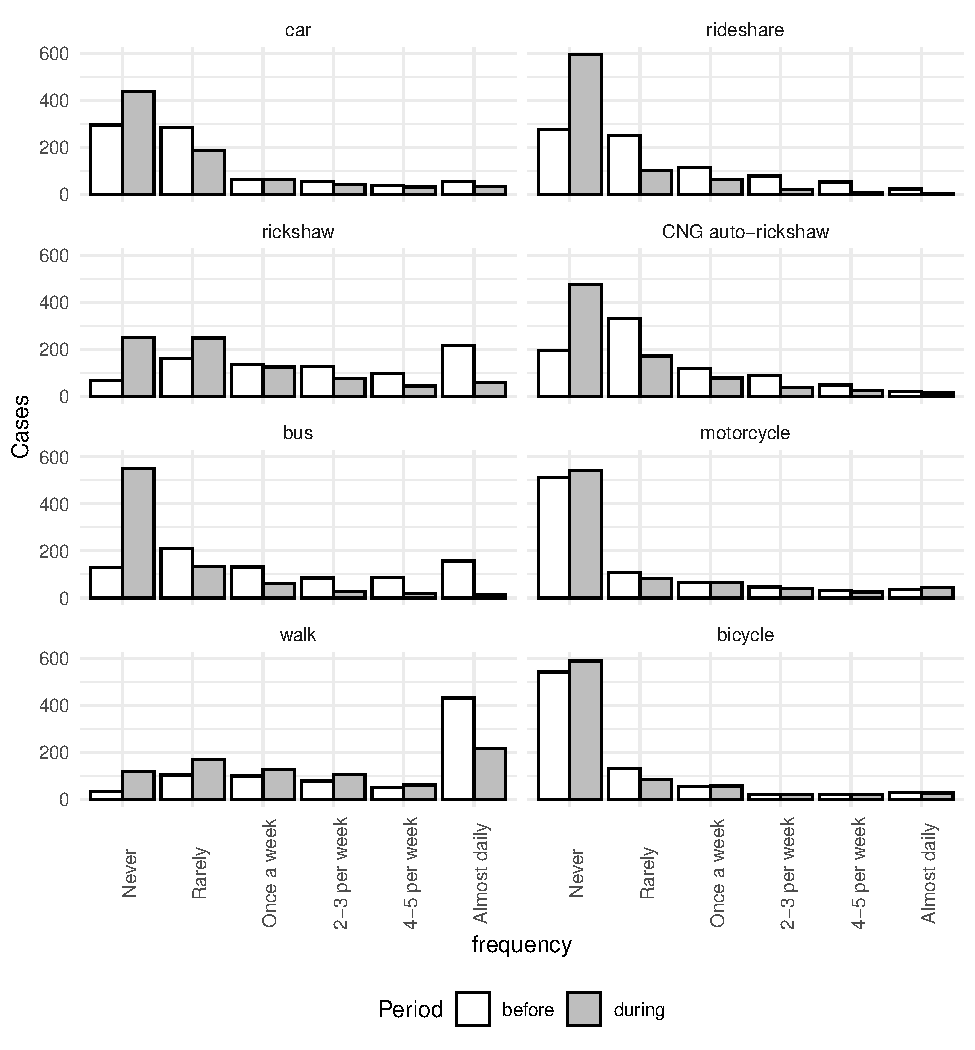
\includegraphics{Frequency-of-Travel-by-Mode-COVID-19-Bangladesh_files/figure-latex/column-plot-cases-before-after-1.pdf}
\caption{\label{fig:column-plot-cases}Number of responses by trip-making
frequency class and mode, before and during COVID-19}
\end{figure}

\begin{table}[H]

\caption{\label{tab:table-transitions}\label{tab:cross-tabulation} Cross-tabulation of counts of travel frequency by mode, before and during COVID-19}
\centering
\resizebox{\linewidth}{!}{
\begin{tabular}[t]{lrrrrrr}
\toprule
  & Never & Rarely & Once a week & 2-3 per week & 4-5 per week & Almost daily\\
\midrule
\addlinespace[0.3em]
\multicolumn{7}{l}{\textbf{car}}\\
\hspace{1em}Never & 267 & 20 & 5 & 1 & 1 & 2\\
\hspace{1em}Rarely & 142 & 99 & 21 & 12 & 9 & 3\\
\hspace{1em}Once a week & 11 & 23 & 19 & 7 & 2 & 3\\
\hspace{1em}2-3 per week & 10 & 23 & 7 & 6 & 8 & 2\\
\hspace{1em}4-5 per week & 4 & 9 & 5 & 6 & 12 & 4\\
\hspace{1em}Almost daily & 6 & 15 & 6 & 10 & 0 & 20\\
\addlinespace[0.3em]
\multicolumn{7}{l}{\textbf{rideshare}}\\
\hspace{1em}Never & 254 & 13 & 6 & 4 & 0 & 0\\
\hspace{1em}Rarely & 192 & 44 & 12 & 1 & 1 & 1\\
\hspace{1em}Once a week & 60 & 20 & 31 & 3 & 1 & 0\\
\hspace{1em}2-3 per week & 49 & 12 & 9 & 7 & 2 & 0\\
\hspace{1em}4-5 per week & 28 & 10 & 3 & 5 & 6 & 2\\
\hspace{1em}Almost daily & 14 & 3 & 4 & 1 & 0 & 2\\
\addlinespace[0.3em]
\multicolumn{7}{l}{\textbf{rickshaw}}\\
\hspace{1em}Never & 51 & 9 & 6 & 0 & 1 & 0\\
\hspace{1em}Rarely & 64 & 70 & 18 & 4 & 3 & 1\\
\hspace{1em}Once a week & 36 & 38 & 45 & 9 & 3 & 3\\
\hspace{1em}2-3 per week & 34 & 36 & 18 & 29 & 6 & 4\\
\hspace{1em}4-5 per week & 21 & 30 & 7 & 16 & 15 & 8\\
\hspace{1em}Almost daily & 45 & 65 & 30 & 18 & 16 & 41\\
\addlinespace[0.3em]
\multicolumn{7}{l}{\textbf{CNG auto-rickshaw}}\\
\hspace{1em}Never & 176 & 14 & 3 & 1 & 0 & 0\\
\hspace{1em}Rarely & 213 & 95 & 14 & 4 & 1 & 3\\
\hspace{1em}Once a week & 36 & 31 & 38 & 9 & 2 & 3\\
\hspace{1em}2-3 per week & 29 & 18 & 16 & 14 & 8 & 3\\
\hspace{1em}4-5 per week & 13 & 6 & 5 & 9 & 14 & 1\\
\hspace{1em}Almost daily & 8 & 7 & 2 & 0 & 0 & 4\\
\addlinespace[0.3em]
\multicolumn{7}{l}{\textbf{bus}}\\
\hspace{1em}Never & 116 & 9 & 3 & 0 & 0 & 0\\
\hspace{1em}Rarely & 155 & 46 & 9 & 0 & 0 & 1\\
\hspace{1em}Once a week & 73 & 32 & 22 & 4 & 0 & 0\\
\hspace{1em}2-3 per week & 43 & 19 & 11 & 7 & 5 & 0\\
\hspace{1em}4-5 per week & 60 & 6 & 5 & 4 & 12 & 1\\
\hspace{1em}Almost daily & 103 & 21 & 10 & 11 & 2 & 10\\
\addlinespace[0.3em]
\multicolumn{7}{l}{\textbf{motorcycle}}\\
\hspace{1em}Never & 467 & 22 & 12 & 3 & 1 & 8\\
\hspace{1em}Rarely & 44 & 38 & 13 & 10 & 0 & 4\\
\hspace{1em}Once a week & 11 & 11 & 34 & 3 & 3 & 3\\
\hspace{1em}2-3 per week & 13 & 6 & 6 & 15 & 4 & 2\\
\hspace{1em}4-5 per week & 6 & 4 & 0 & 4 & 14 & 3\\
\hspace{1em}Almost daily & 1 & 3 & 2 & 4 & 3 & 23\\
\addlinespace[0.3em]
\multicolumn{7}{l}{\textbf{walk}}\\
\hspace{1em}Never & 17 & 7 & 3 & 4 & 0 & 2\\
\hspace{1em}Rarely & 26 & 53 & 13 & 6 & 2 & 4\\
\hspace{1em}Once a week & 12 & 19 & 54 & 9 & 4 & 2\\
\hspace{1em}2-3 per week & 10 & 14 & 12 & 26 & 13 & 4\\
\hspace{1em}4-5 per week & 7 & 3 & 7 & 11 & 16 & 8\\
\hspace{1em}Almost daily & 46 & 73 & 40 & 49 & 27 & 197\\
\addlinespace[0.3em]
\multicolumn{7}{l}{\textbf{bicycle}}\\
\hspace{1em}Never & 504 & 22 & 7 & 4 & 2 & 4\\
\hspace{1em}Rarely & 59 & 43 & 20 & 4 & 2 & 4\\
\hspace{1em}Once a week & 14 & 13 & 21 & 3 & 2 & 1\\
\hspace{1em}2-3 per week & 3 & 4 & 5 & 7 & 2 & 0\\
\hspace{1em}4-5 per week & 2 & 2 & 4 & 1 & 9 & 3\\
\hspace{1em}Almost daily & 7 & 1 & 1 & 1 & 3 & 16\\
\bottomrule
\end{tabular}}
\end{table}

The frequency of trip-making by other modes changed more noticeably: the
frequency of travel by ridesharing services, rickshaw, CNG
auto-rickshaw, and bus collapsed, with vastly more respondents reporting
never using these modes during the pandemic than before. The frequency
of walking trips also decreased (fewer respondents report walking almost
daily), but the reductions in mobility were not so heavily concentrated
at the bottom of the scale.

Table \ref{tab:cross-tabulation} is a cross-tabulation of the number of
cases in each trip-making frequency class before and during the
pandemic. If no changes had occurred, all values would be concentrated
on the main diagonal of the matrices. Values in the lower triangular
matrix represent a \emph{loss} of mobility (lower travel frequency),
whereas values in the upper triangular matrix are \emph{gains} (higher
travel frequency). The further away a value is from the main diagonal,
the greater the loss or gain.

Despite across-the-board losses of mobility, there appears to have been
some adaptation that varied by mode of transportation. To illustrate,
103 respondents, or 65.61\% of those who traveled by bus almost daily
before, reported never using it during the pandemic. In contrast, only
12 respondents, or 1.5\% of those who never used buses before started
doing so during the pandemic. By way of comparison, 24.14\% of
respondents who cycled almost daily before the pandemic stopped doing so
- but 4.88\% who never cycled before started doing so during the
pandemic.

To more clearly understand the transitions towards different trip-making
frequencies, including possible adaptations, we convert the
cross-tabulations to probability transition matrices, which we then
visualize using circular plots.

Figures \ref{fig:circular-plot-1} to \ref{fig:circular-plot-4} present
these plots. Each of the trip-making frequency sectors on the left
hemisphere of the circle represents 100\% of responses \emph{before} the
pandemic. The links' size is proportional to the probability \(p_{ij}\)
of transitioning from frequency class \(i\) before to the right
hemisphere are proportional to the transition probabilities to each
frequency \emph{during} the pandemic. There are three transparency
levels for the links: solid colors are for \(p_{ij}>2/3\), intermediate
transparency is for \(1/3 < p_{ij} \le 2/3\), and the more transparent
links are for \(p_{ij}\le 1/3\).

From Figure \ref{fig:circular-plot-1}, we see that the probability of
traveling less by car for those who initially used this mode frequently
is high, but their probability of not using this mode at all during the
pandemic is quite small. In other words, there was a decline in use, but
not complete discontinuation of this mode. The probability of traveling
more frequently by car for those who originally never or rarely used
this mode remained is low. In contrast, we see that the probabilities of
never ridesharing during the pandemic are high irrespective of the
initial level of use of this mode of transportation, and the probability
of using this mode more are fairly small.

\begin{figure}
\centering
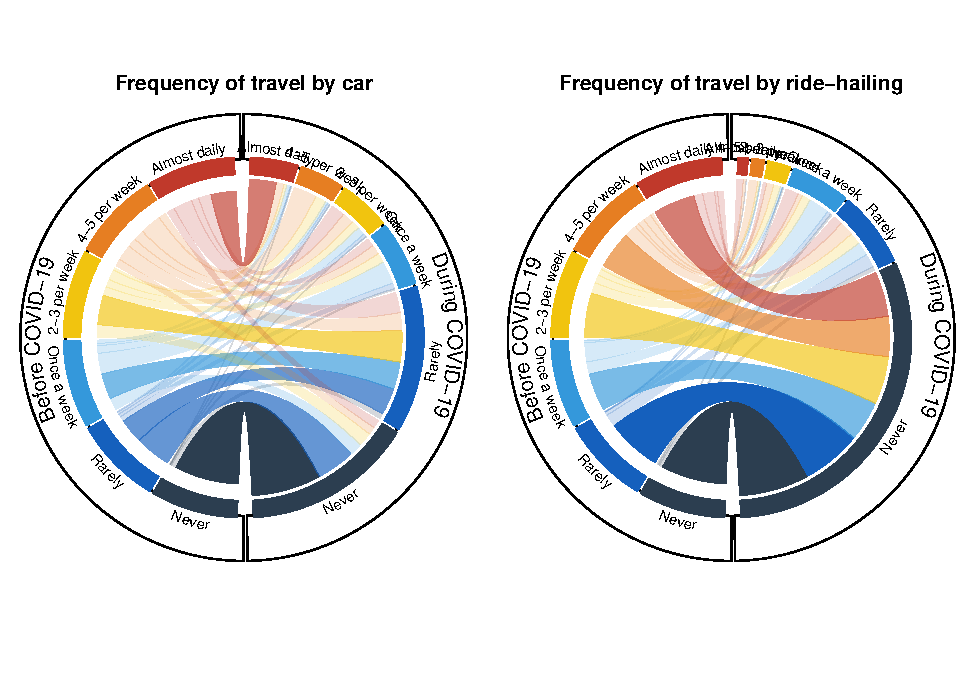
\includegraphics{Frequency-of-Travel-by-Mode-COVID-19-Bangladesh_files/figure-latex/circular-plots-transition-probabilities-1-1.pdf}
\caption{\label{fig:circular-plot-1}Transition probabilities in trip
frequency from before to during COVID-19: car and rideshare}
\end{figure}

The probabilities of change in trip frequency by rickshaw and CNG
auto-rickshaw are similar (see Figure \ref{fig:circular-plot-2}),
although the probabilities of being less mobile by CNG auto-rickshaw are
greater: between 1/3 and 2/3 of respondents who used this mode almost
daily, stopped using it during the pandemic. Very rarely there were
increases in mobility by these modes.

\begin{figure}
\centering
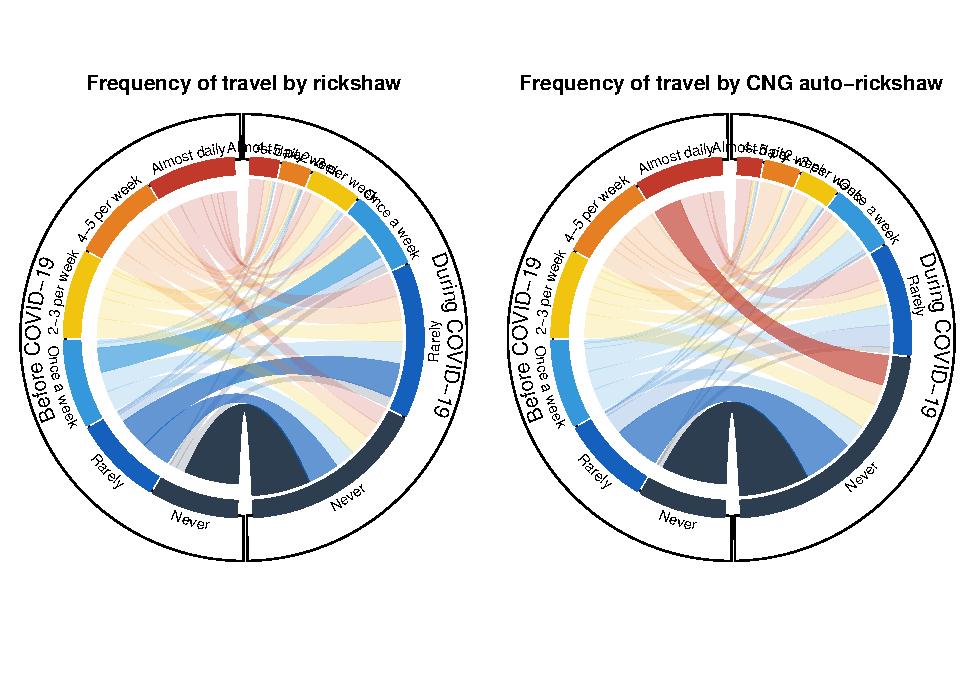
\includegraphics{Frequency-of-Travel-by-Mode-COVID-19-Bangladesh_files/figure-latex/circular-plots-transition-probabilities-2-1.pdf}
\caption{\label{fig:circular-plot-2}Transition probabilities in trip
frequency from before to during COVID-19: rickshaw and cng
auto-rickshaw}
\end{figure}

After rideshare, the use of bus had the largest probabilities of
discontinuation (Figure \ref{fig:circular-plot-3}). We see that even
respondents who used this mode almost daily before the pandemic had
close to 66\% chances of never using it during the contingency.
Similarly large losses of mobility by bus were observed for travelers
who used this mode less frequently before the pandemic. These losses
were not offset to any appreciable degree by the probability of some
users turning to this mode during the pandemic.

\begin{figure}
\centering
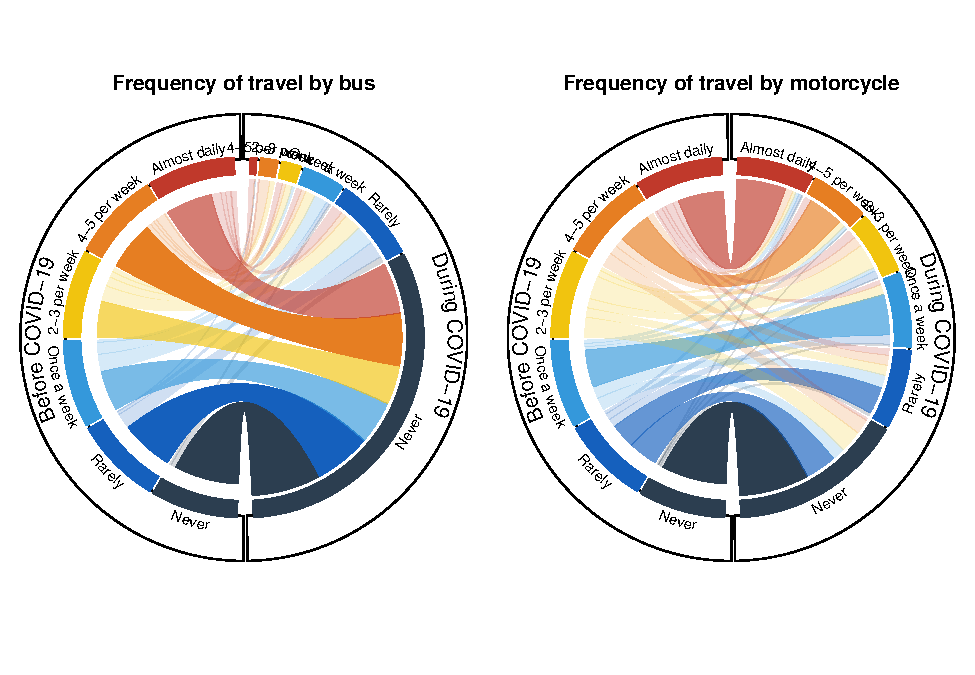
\includegraphics{Frequency-of-Travel-by-Mode-COVID-19-Bangladesh_files/figure-latex/circular-plots-transition-probabilities-3-1.pdf}
\caption{\label{fig:circular-plot-3}Transition probabilities in trip
frequency from before to during COVID-19: motorcycle and bus}
\end{figure}

Trip-making by motorcycle (Figure \ref{fig:circular-plot-3}) also
declined for all but the most frequent users pre-COVID-19, and the
probability of adopting this mode during COVID-19 was almost null.
Contrast this to the case of walking (Figure \ref{fig:circular-plot-4}),
where a sizable number of respondents started walking during the
pandemic, even if only rarely. Close to 50\% of respondents who report
walking almost daily during the pandemic walked less frequently before
the contingency. Bicycle (Figure \ref{fig:circular-plot-4}), like
motorcycle, saw relatively fewer respondents adopting it during the
pandemic, and many travelers who did use the mode rarely, once a week,
or even 2-3 times per week stopped cycling during the pandemic.

\begin{figure}
\centering
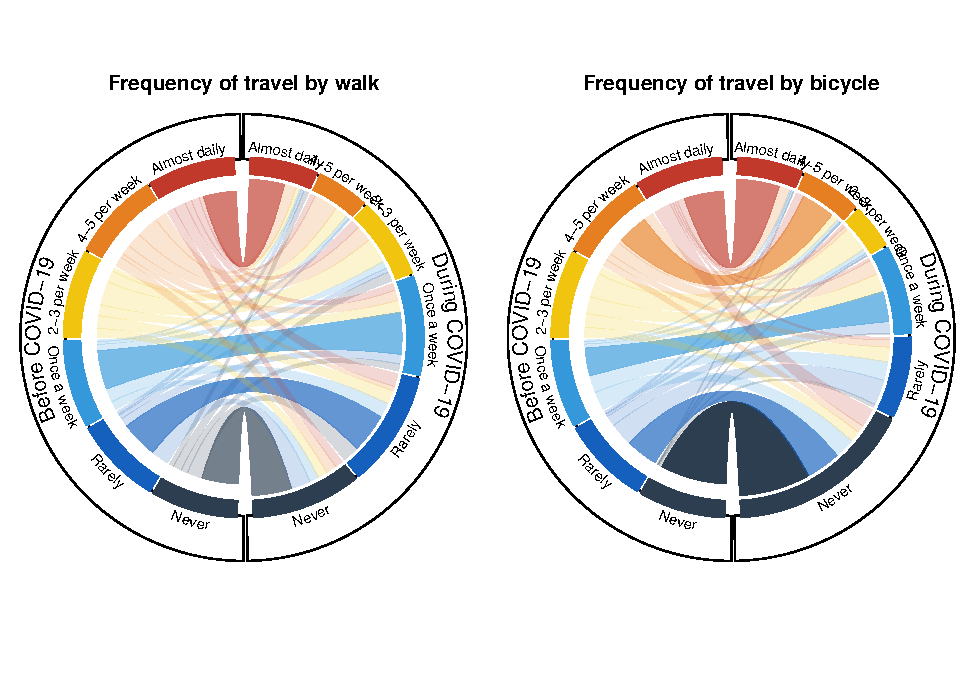
\includegraphics{Frequency-of-Travel-by-Mode-COVID-19-Bangladesh_files/figure-latex/circular-plots-transition-probabilities-4-1.pdf}
\caption{\label{fig:circular-plot-4}Transition probabilities in trip
frequency from before to during COVID-19: bicycle and walk}
\end{figure}

The findings reported here provide important changes in mobility in a
developing country during COVID-19. In general there was a loss of
mobility across-the-board, but modes that require interaction with
strangers (rideshare, bus, rickshaw, and CNG auto-rickshaw) were more
affected. Travel by car, motorcycle, and bicycle were somewhat less
affected, and there is evidence of some adoption of walking during the
pandemic.

\hypertarget{references}{%
\section*{References}\label{references}}
\addcontentsline{toc}{section}{References}

\hypertarget{refs}{}
\leavevmode\hypertarget{ref-Astroza2020mobility}{}%
Astroza, S., Tirachini, A., Hurtubia, R., Carrasco, J.A., Guevara, A.,
Munizaga, M., Figueroa, M., Torres, V., 2020. Mobility changes,
teleworking, and remote communication during the covid-19 pandemic in
chile. Transport Findings.
doi:\href{https://doi.org/10.32866/001c.13489}{10.32866/001c.13489}

\leavevmode\hypertarget{ref-Brunsdon2020opening}{}%
Brunsdon, C., Comber, A., 2020. Opening practice: Supporting
reproducibility and critical spatial data science. Journal of
Geographical Systems 1--20.

\leavevmode\hypertarget{ref-DeWeese2020tale}{}%
DeWeese, J., Hawa, L., Demyk, H., Davey, Z., Belikow, A., El-geneidy,
A., 2020. A tale of 40 cities: A preliminary analysis of equity impacts
of covid-19 service adjustments across north america. Tansport Findings.
doi:\href{https://doi.org/10.32866/001c.13395}{10.32866/001c.13395}

\leavevmode\hypertarget{ref-Huynh2020culture}{}%
Huynh, T.L.D., 2020. Does culture matter social distancing under the
covid-19 pandemic? Safety Science 130, 7.
doi:\href{https://doi.org/10.1016/j.ssci.2020.104872}{10.1016/j.ssci.2020.104872}

\leavevmode\hypertarget{ref-Lock2020cycling}{}%
Lock, O., 2020. Cycling behaviour changes as a result of covid-19: A
survey of users in sydney, australia. Transport Findings.
doi:\href{https://doi.org/10.32866/001c.13405}{10.32866/001c.13405}

\leavevmode\hypertarget{ref-Molloy2020tracing}{}%
Molloy, J., Tchervenkov, C., Hintermann, B., Axhausen, K.W., 2020.
Tracing the sars-cov-2 impact: The first month in switzerland. Transport
Findings.
doi:\href{https://doi.org/10.32866/001c.12903}{10.32866/001c.12903}

\leavevmode\hypertarget{ref-Paez2020using}{}%
Paez, A., 2020. Using google community mobility reports to investigate
the incidence of covid-19 in the united states. Transport Findings.
doi:\href{https://doi.org/10.32866/001c.12976}{10.32866/001c.12976}

\leavevmode\hypertarget{ref-Saha2020lockdown}{}%
Saha, J., Barman, B., Chouhan, P., 2020. Lockdown for covid-19 and its
impact on community mobility in india: An analysis of the covid-19
community mobility reports, 2020. Children and Youth Services Review
116, 14.
doi:\href{https://doi.org/10.1016/j.childyouth.2020.105160}{10.1016/j.childyouth.2020.105160}


\end{document}


